%----------------------------------------------------------------------------
\appendix
%----------------------------------------------------------------------------
\chapter*{\fuggelek}\addcontentsline{toc}{chapter}{\fuggelek}
\setcounter{chapter}{\appendixnumber}
%\setcounter{equation}{0} % a fofejezet-szamlalo az angol ABC 6. betuje (F) lesz
\numberwithin{equation}{section}
\numberwithin{figure}{section}
\numberwithin{lstlisting}{section}
%\numberwithin{tabular}{section}

%----------------------------------------------------------------------------
\section{Az esettanulmányhoz készített támadási fák}
%----------------------------------------------------------------------------
\begin{figure}[!ht]
\centering
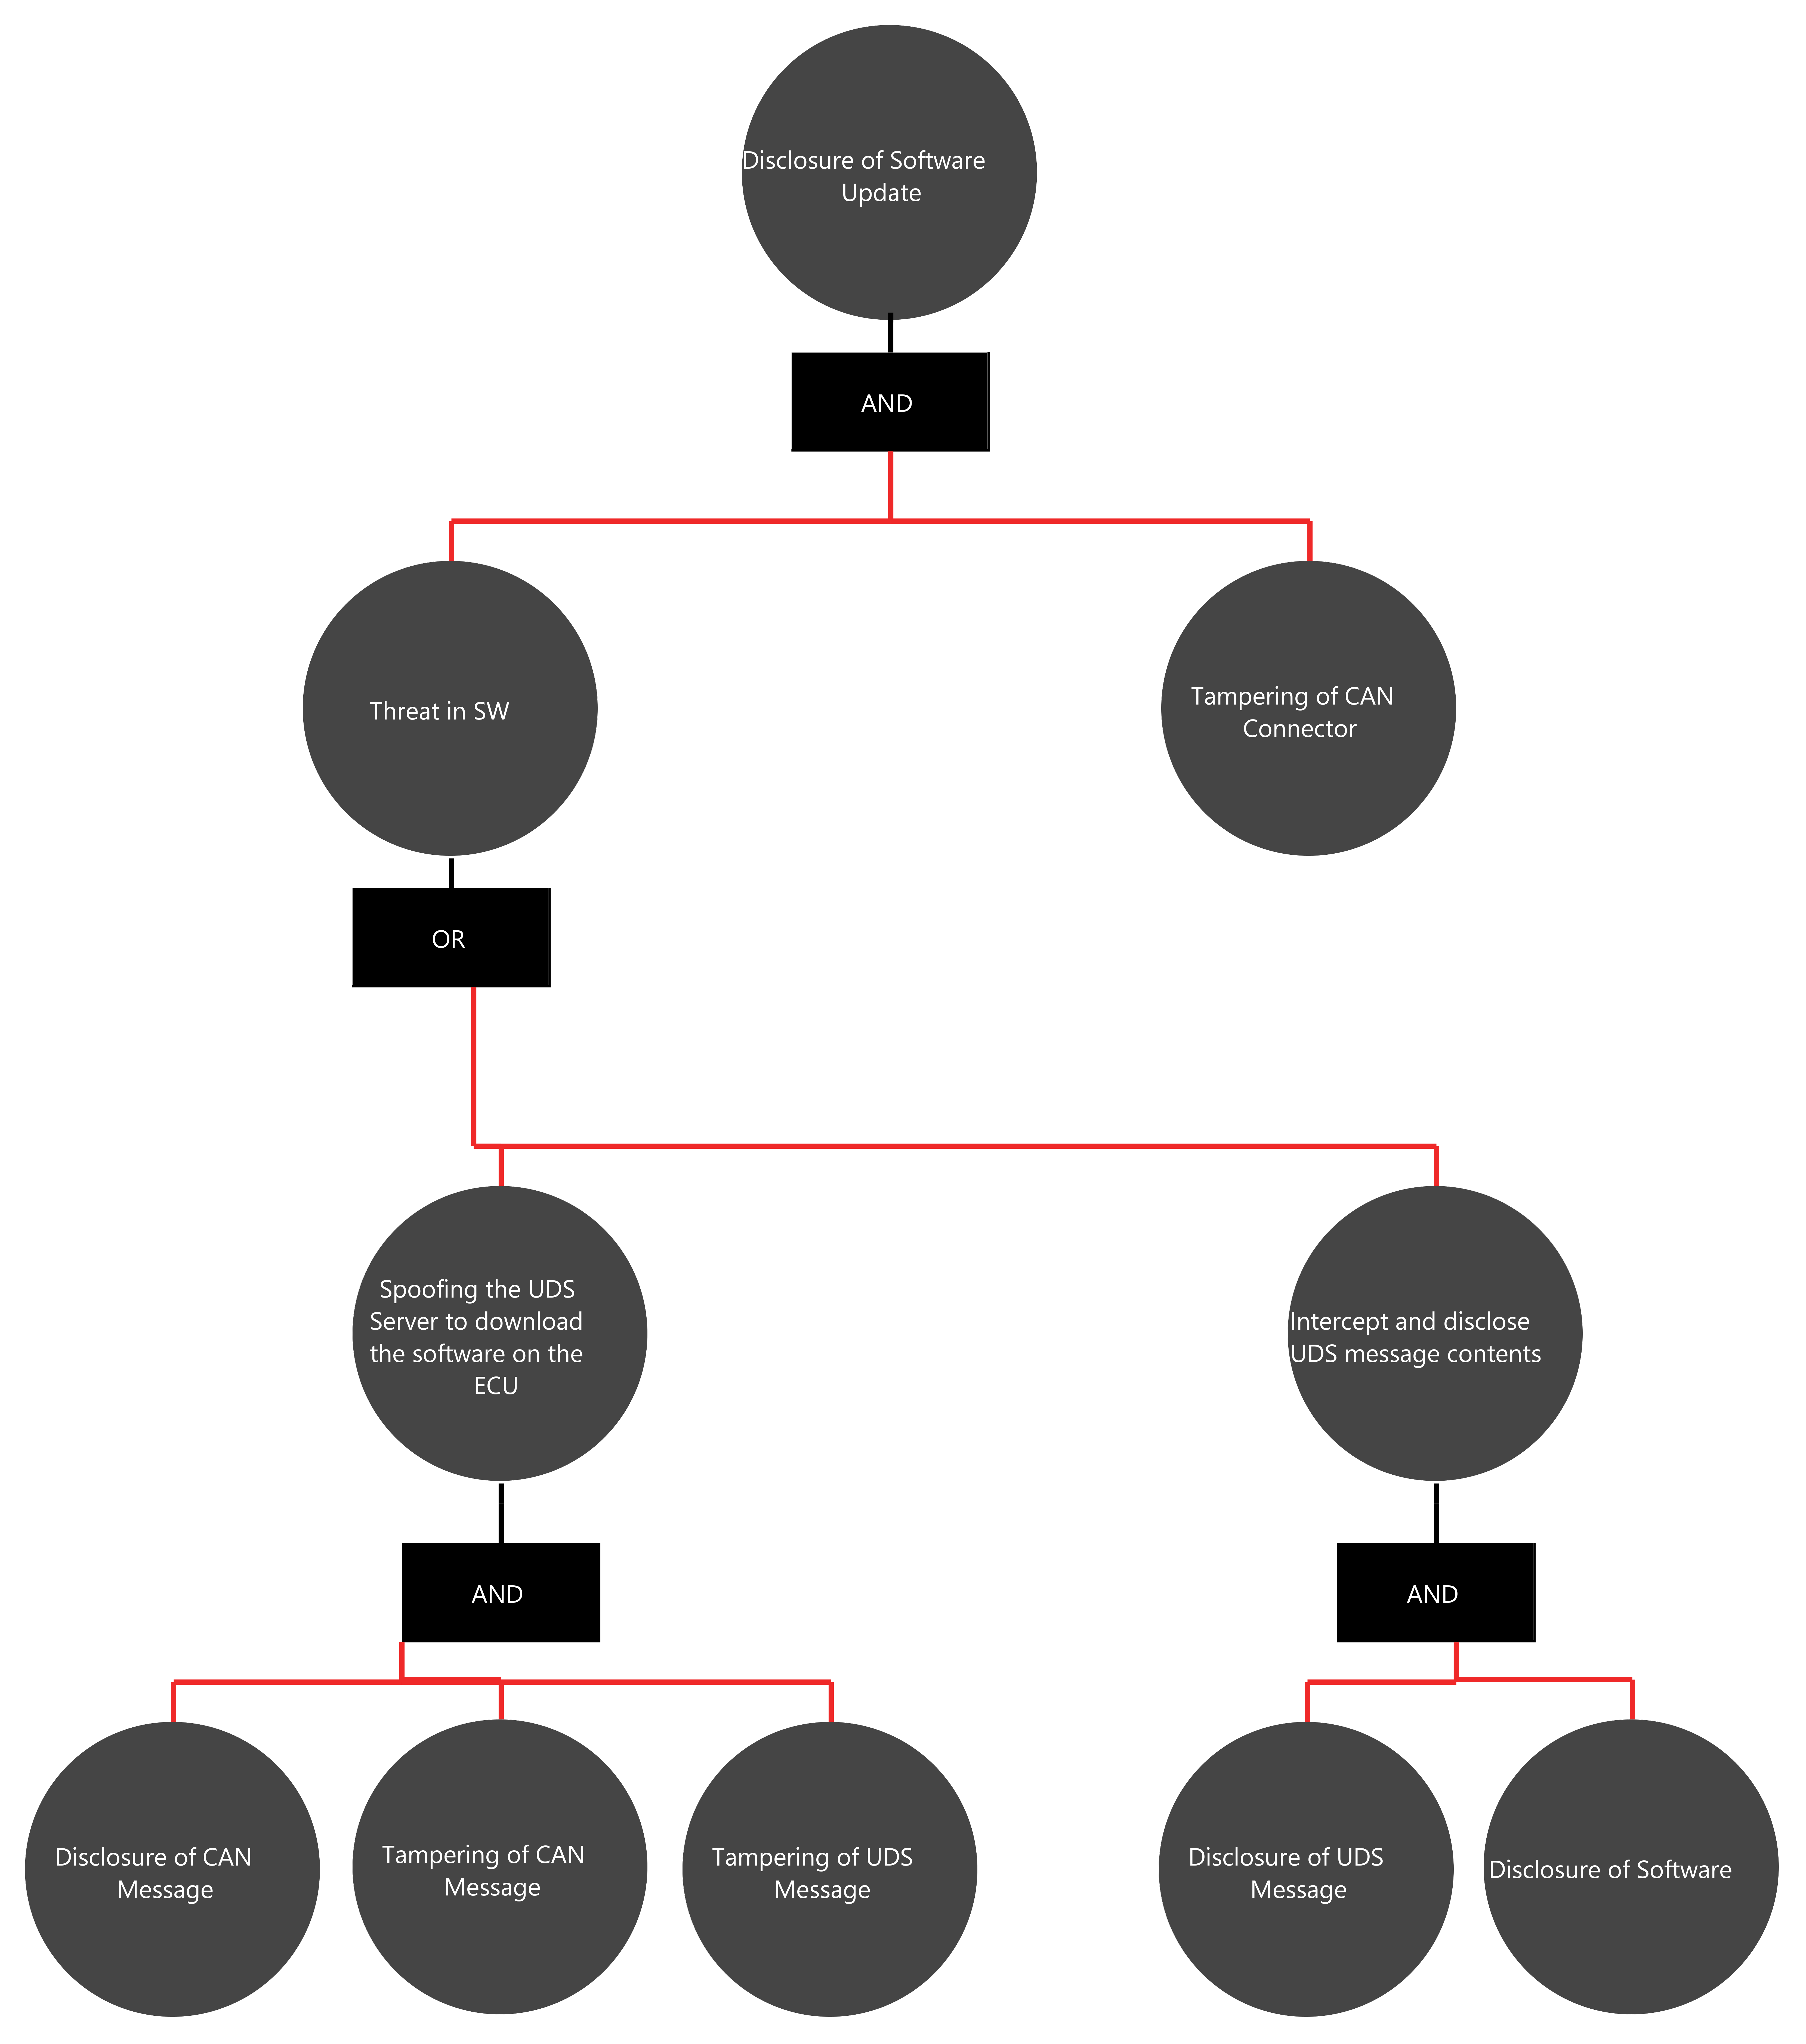
\includegraphics[width=120mm, keepaspectratio]{figures/AT-SECSW-00.png}
\caption{Támadási fa a "Leak software" károkozáshoz} 
\label{fig:ff_leak_sw}
\end{figure}
